\documentclass[60pt]{article}
\usepackage{babel}
\usepackage[T1]{fontenc}
\usepackage{textcomp}
\usepackage[utf8]{inputenc}
\usepackage{enumerate}
\usepackage{graphicx}
\graphicspath{ {imagenes/} }


\title{\textbf{Universidad Veracruzana}}
\date{\textbf{Facultad de Negocios y Tecnologías}}


\begin{document}

\maketitle
\begin{figure}[htb]
\centering

\includegraphics[width=0.5\linewidth]{logo.png}
\end{figure}

\maketitle
\textsf{\Large 
\\
\\
\textbf{EXPERIENCIA EDUCATIVA:} Bases De Datos No Convencional. \\}
\\
\\ 
\maketitle
\textsf{\Large \textbf{ACADÉMICO:} Centeno Tellez Adolfo. \\}
\\
\\
\maketitle
\textsf{\Large \textbf{Proyecto:} Pinterest con firebase y firestore. \\}
\\
\\
\maketitle
\textsf{\Large \textbf{ESTUDIANTE:} Hernandez Sanchez Jesus Gabriel. \\}
\\
\\ 
\maketitle
\textsf{\Large \textbf{GRUPO:} 601 - Ingeniería de Software \\}
\\
\\

\newpage

\section{Introducción}

El siguiente documento describirá de manera resumida el proyecto de crear una aplicacion web que se asemeja de manera muy sencilla a la famosa aplicacion de Pinterest, usando bases de datos no relacionales usando como herramienta a firebase y firestore. Tambien usando a Facebook como login de la misma.

\subsection{Objetivos del proyecto}
El proyecto se hizo con el objetivo de poner en practica el uso y entendimiento de las bases de datos no convencionales que a dia de hoy son de las mas usadas en un dia a dia, tomando como ejemplo a las redes sociales en donde todos los dias se suben imagenes, videos, gifts,etc. 

\section{Descripción del proyecto}
El proyecto es una aplicacion que hace referencia a Pinterest, aplicacion para ver y subir imagenes, esta se lleva a cabo usando algunas tecnologias como lo son React y Rirebase/Firestore, tambien se usa Facebook como metodo de autentificacion, otra herramienta es bootstrap para facilitar el front de la aplicacion.

A continuacion se anexaran capturas de pantalla de la pagina y de su funcionamiento.

\subsection{Ingresar con Facebook}

En esta pantalla el usuario tiene que ingresar con su cuenta de facebook

\begin{figure}[htb]
\centering
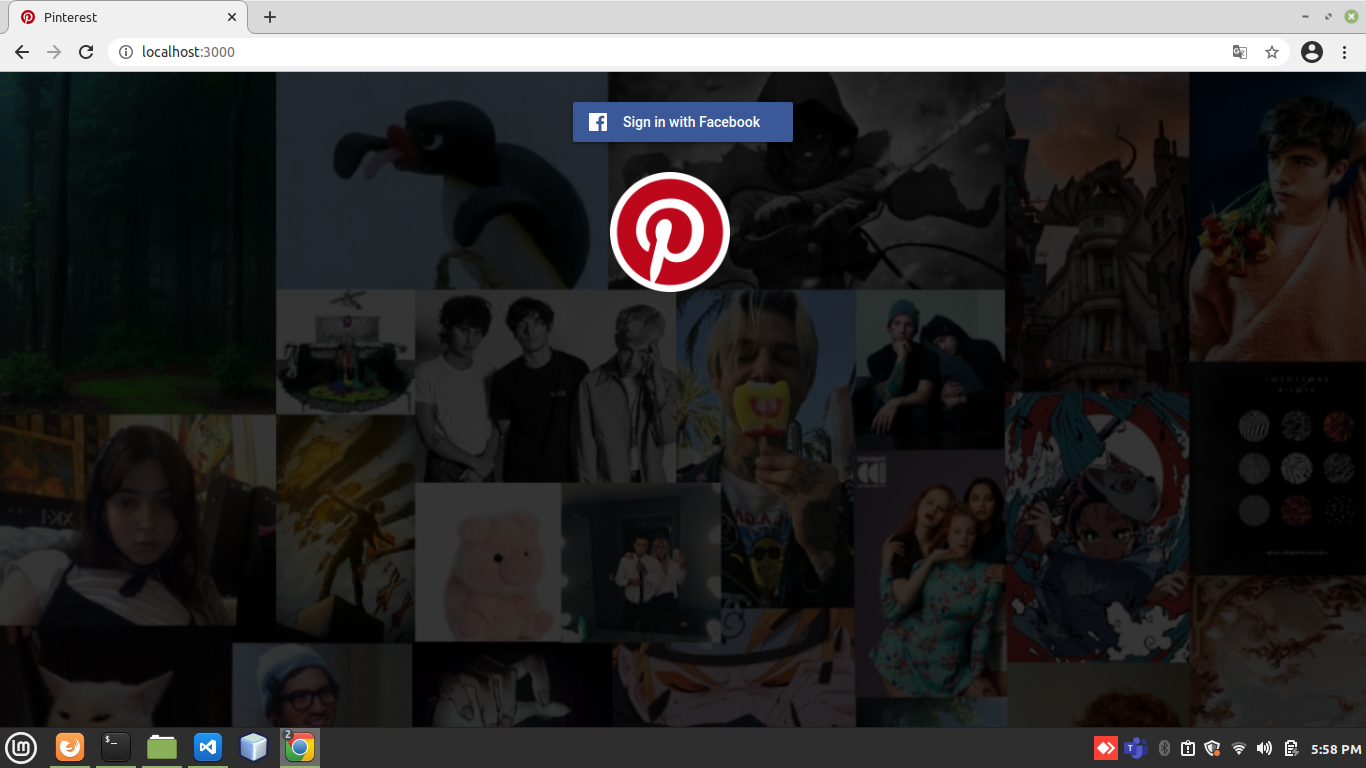
\includegraphics[width=1\linewidth]{facebook.png}
\end{figure}

\subsection{Cuenta logueada en Firebase}
Aqui se muestra como la cuenta fue añadida al apartado de autentificacion de firebase
\begin{figure}[htb]
\centering
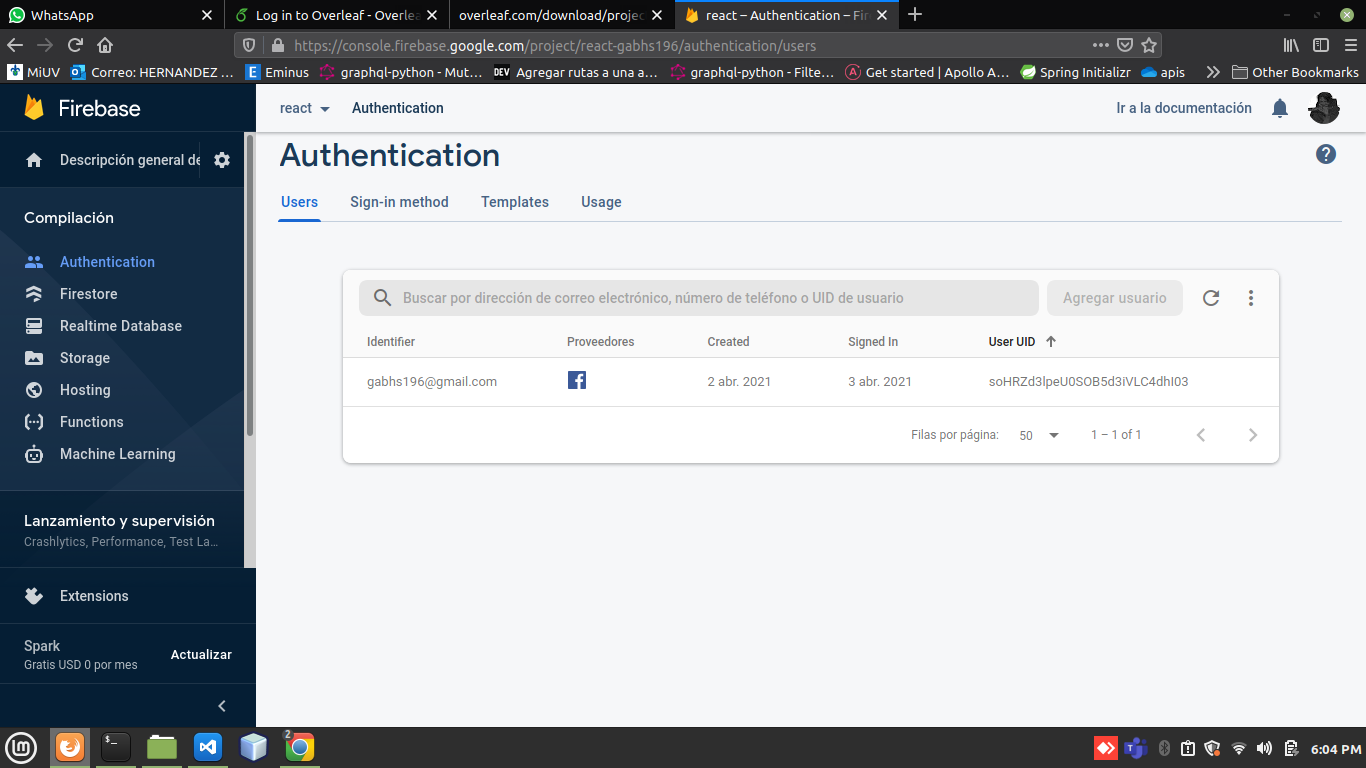
\includegraphics[width=1\linewidth]{autenticacion.png}
\end{figure}

\subsection{Pantalla principal}
Esta es la pantalla principal de la aplicacion, que cuenta con un banner en donde se muestra la foto de perfil y nombre en Facebook de la persona que se logueó, acompañado de un boton de salir que cierra la sesion. Abajo se muestra un boton para subir una imagen que se mostrara segundos mas tarde en la parte de abajo
\begin{figure}[htb]
\centering
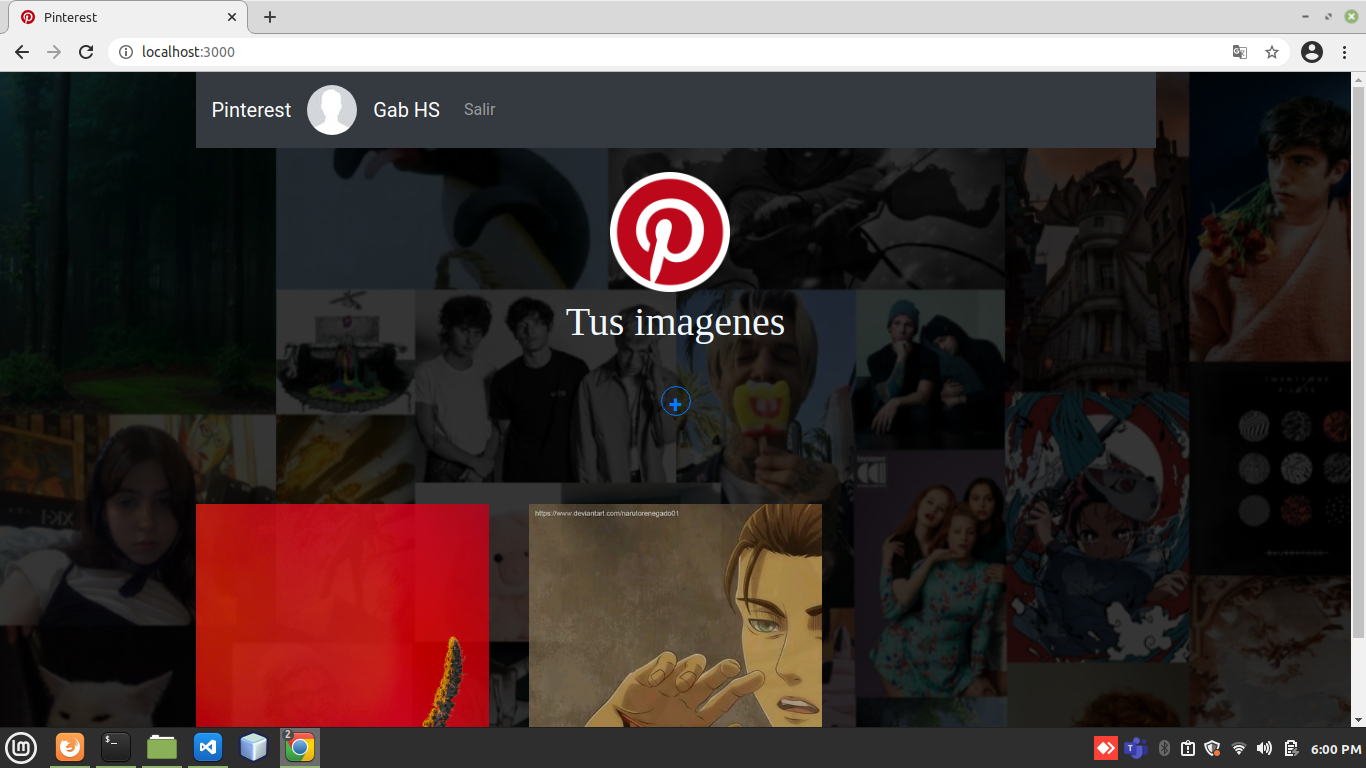
\includegraphics[width=.94\linewidth]{principal.png}
\end{figure}

\subsection{Agregar imagen}
Si damos click en el icono de mas, podemos agregar una imagen
\begin{figure}[htb]
\centering
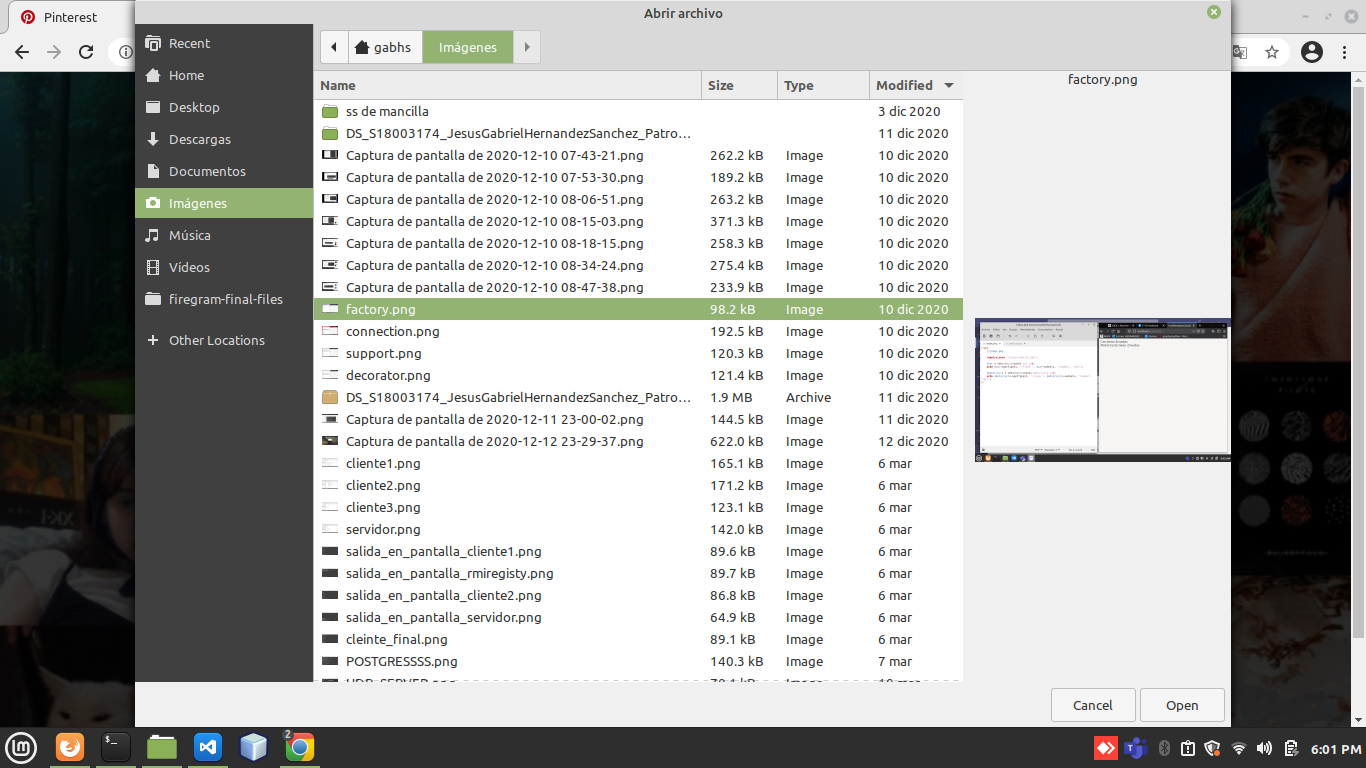
\includegraphics[width=1\linewidth]{agregar.png}
\end{figure}

\subsection{Imagen agregada}
La imagen ya se encuentra en la parte de abajo
\begin{figure}[htb]
\centering
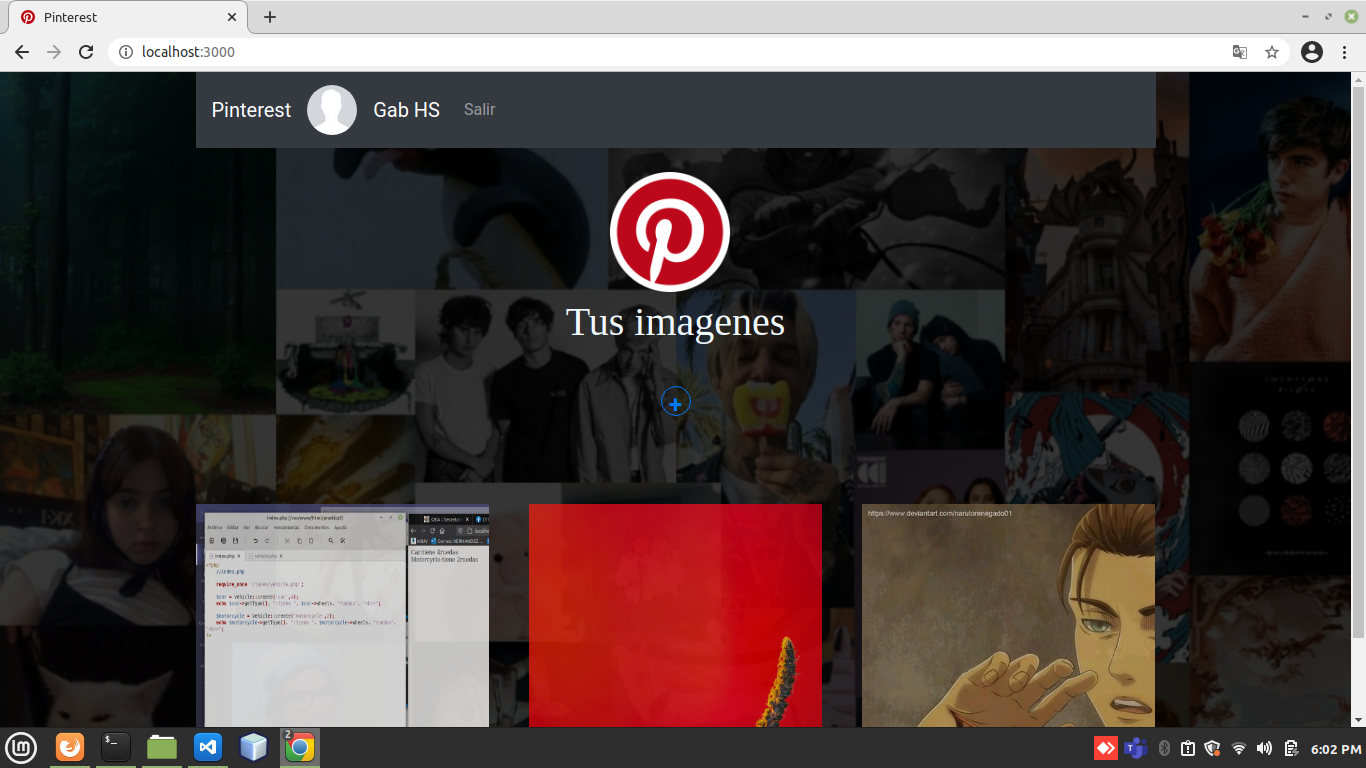
\includegraphics[width=1\linewidth]{imagenAgregada.png}
\end{figure}

\newpage
\subsection{Imagen agrandada}
Si damos click en la imagen se puede agrandar para verla mejor
\begin{figure}[htb]
\centering
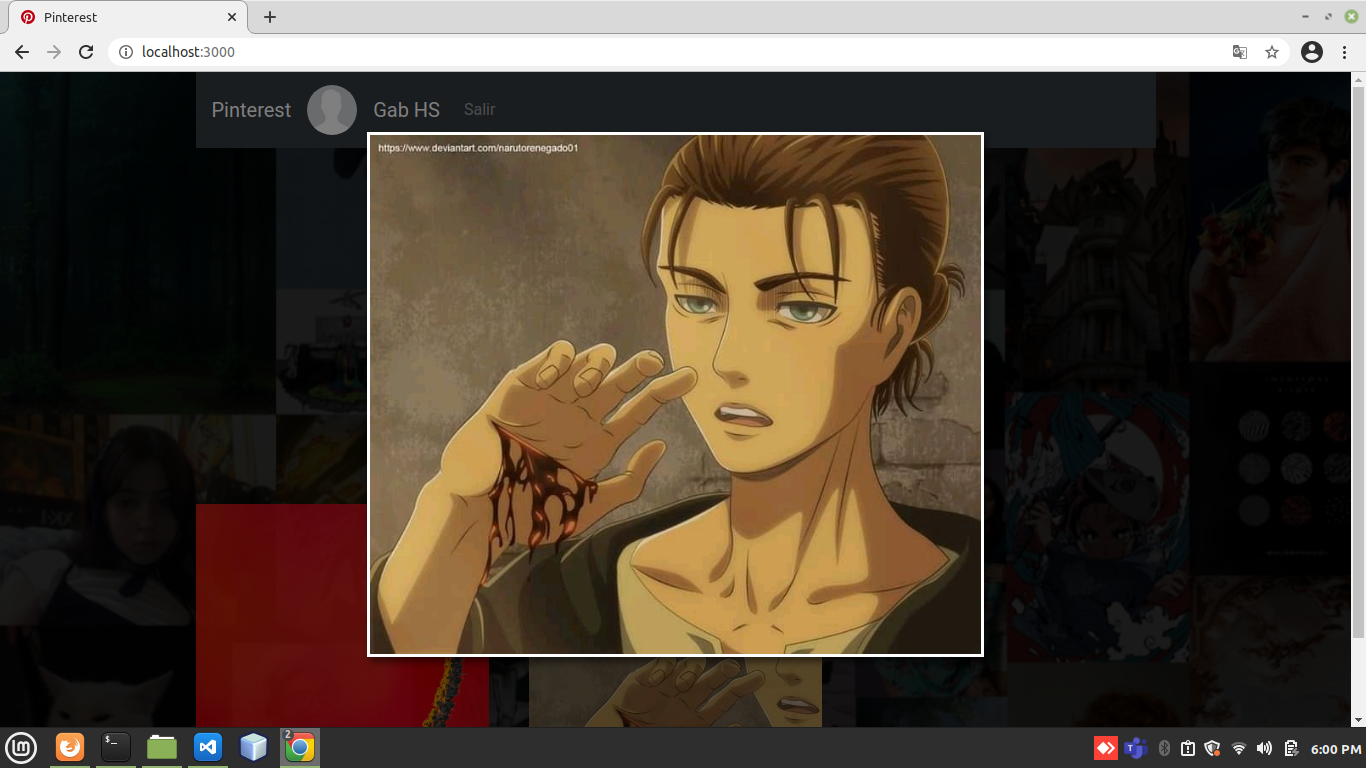
\includegraphics[width=1\linewidth]{imagenGrande.png}
\end{figure}

\subsection{Storage}
Aqui se muestran las imagenes cargadas en el storage de firebase
\begin{figure}[htb]
\centering
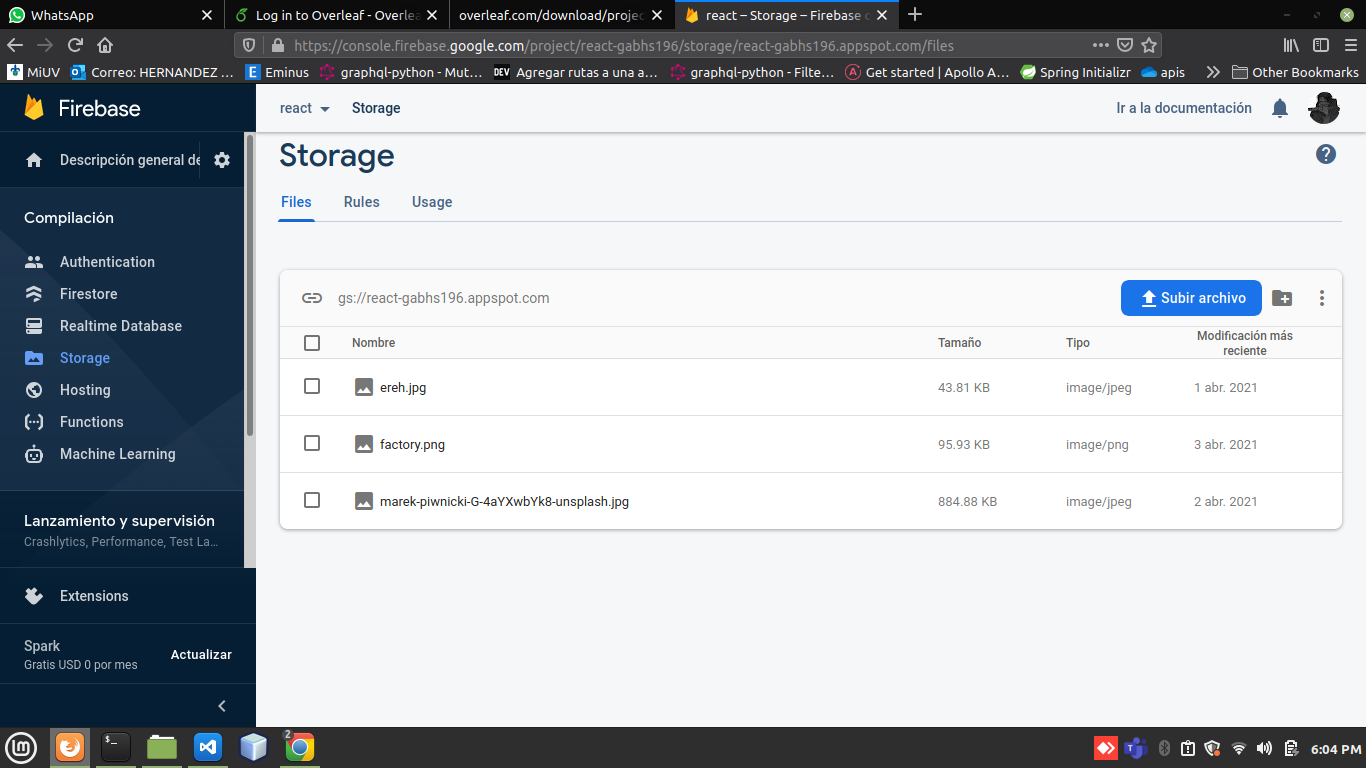
\includegraphics[width=1\linewidth]{storage.png}
\end{figure}

\subsection{Firestore}
Aqui se puede ver la coleccion de imagenes con su url y un dato de fecha para conocer en que fecha fue agregada
\begin{figure}[htb]
\centering
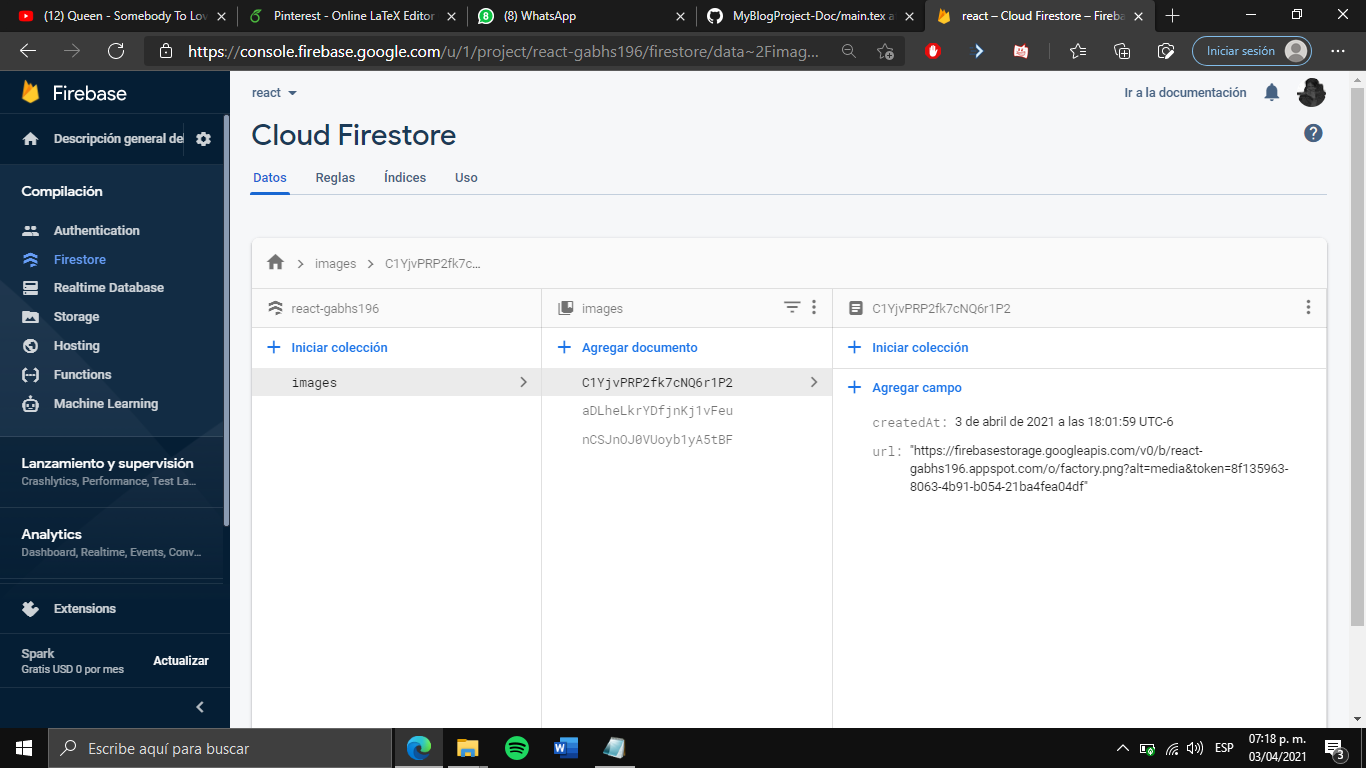
\includegraphics[width=1\linewidth]{firestore.png}
\end{figure}

\section{Conclusión}
En conclusion, esta actividad me sirvio para conocer lo que era una base de datos no convencional, su funcionalidad y como se implementa en una aplicacion web. Y saber que no solamente existen las bases de datos relacionales como MySql,Postgres,etc. Las bases de datos no convencionales están en todas partes y son sumamente importantes en el dia a dia de cualquier persona.

\end{document}
